\chapter{Background}
\label{background}
\section{Infandango}
Infandango is an automated web-based marking system for student submitted programming exercises. A student can view the list of warm-up, optional and core exercises and choose to submit a file for one of them. This file is then compiled and tested by Jester in a sandbox. Between the web frontend and Jester there is a PostgresSQL database which stores the source code of each submission and the score information for each marked submission.
Each question has a label: {\bf warmup} questions are simple questions which can be skipped if the user feels confident, {\bf core} questions are questions which the user is highly encouraged to try and may affect the end coursework mark, and {\bf optional} questions are provided for particularly interested students.
\subsection{Current feedback}
The primary source of feedback in Infandango is displayed in Figure \ref{fig:currentfeedback}. Each submission is marked with a set of JUnit tests and the fraction of these tests which are correct is displayed. This fraction is converted into a percentage and displayed on a red (0 - 40\%), orange (40\%-70\%) or green (70\%-100\%) background.
More general feedback is also available which displays similar information but the results are displayed by week rather than by question. 

\begin{figure}[h!]
\centering
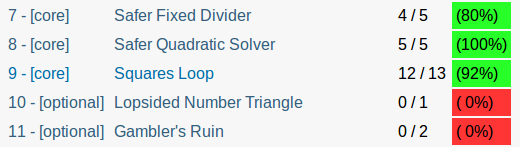
\includegraphics[width=0.8\textwidth]{images/currentfeedback.png}
\caption{This is a cropped screenshot of what is displayed to the user for a given week in the current Infandango system}
\label{fig:currentfeedback}
\end{figure}

\subsection{Current data}
The system has been used with the first year Java programming course at the University of Edinburgh for a few years. The database information for these years has been kept and retains all the information about submissions: marks, submission time, number of resubmissions. The database for one year has been anonymised and made available for use for this project. Only one year is available because the questions have changed since previous years and therefore the data would be inconsistent with the current questions.

\section{Literature}

Khan Academy\cite{khan_site} is a website which provides users with online education material:
\begin{quote}
Our online materials cover subjects ranging from math and finance to history and art.  With thousands of bite-sized videos, step-by-step problems and instant data\cite{ka_faq}
\end{quote}

%PUT IMAGE HERE FOR THE PARAGRAPH BELOW

A blog post\cite{khan_blog} written by David Hu about Khan Academy demonstrates that different feedback measures can affect user performance significantly. Khan Academy gives users certain kinds of exercises, for example choosing the approriate position on a number scale. It can then generate endless variations of this problem for the user to continue attempting until they are deemed proficient\footnote{
proficiency is achieved when it is deemed appropriate for a user to move on to other questions
}. The original Khan Academy system required a user to get 10 consecutive exercises of a certain type correct before they are qualified as proficient for that type of exercise. 

The main problem with this system is that a user could get 9 consecutive exercises correct and then make a mistake on the final exercise. Before the user could move on they would have to get 10 more consecutive exercises correct. It would be better if the system took into account how the user had performed previously. 

In an attempt to improve this system Hu proposed using a logistic regression model to calculate the probability that a user passes the next exercise successfully, with a threshold of 94\% representing the new proficiency level. Over a 6 day period 10\% of users tested the new method. Users of the new system earned 20.8\% more proficiences, attempted 15.7\% more exercises and required 26\% less exercises per proficiency. Hu summarises by saying the boost seems to come from allowing users to move on from exercises which they are already proficient at, without requiring them to complete their streak.
Although the current system does not require perfection like Khan Academy did, it is possible that users are more reluctant to move on from exercises before they achieve 100\%. Infandango also lacks any cumulative feedback for a series of exercises. Providing feedback similar to the new Khan Academy approach could provide encouragement for the user to move on.

\subsection{Programming Assessment}
In {\it Automated Evaluation of Programming Assignments}\cite{automate_evaluation}, Kaushal and Singh describe various measures used as part of an automated marking system: regularity, integrity, efficiency and accuracy. 
\paragraph*{Regularity} The time at which a submission is made with respect to the deadline for that submission
\paragraph*{Integrity} The originality of the document determined through a plagiarism detector
\paragraph*{Efficiency} A qualitative measure of the time taken and memory used by a student's programs
\paragraph*{Accuracy} The percentage of test cases for each program that the student's submission passes

Infandango only gives feedback on one of these areas: accuracy. The experimenters track the change in these measures as students use the system and find that there is a general improvement on all categories when feedback is based on these measurements. This shows that accuracy is not the only measurement that should be used to provide feedback and these are possibilities to be considered for Infandango.

\subsection{Visualisation}
In his book {\it Visual Display of Quantitative Information}\cite{visual_explanations}, Edward Tufte discusses methods of efficiently and suitably displaying information. In chapter 4 Data-Ink and Graphical Redesign, Tufte introduces the idea of Data-Ink: The amount of "ink" which is actually used to represent the data you are interested in. In Tufte's words:

\begin{quote}Data-ink is the non-erasable core of a graphic, the non-redundant ink arranged in reponse to the variation in the numbers represented.
\end{quote}
Data-ink is desirable, unavoidable information so designers should strive towards a high data-ink ratio, removing as much non-information ink as possible to avoid overwhelming the data. Tufte then continues by giving examples where redundant information is desirable.
Tufte takes a graphic from Linus Pauling's General Chemistry (San Francisco, 1947) p64. Figure \ref{fig:tuftegraphs} shows how, based on the low data-ink ratio principle, he removes the grid marks and part of the frame which leaves little else but the data itself.

\begin{figure}[h!]
\centering
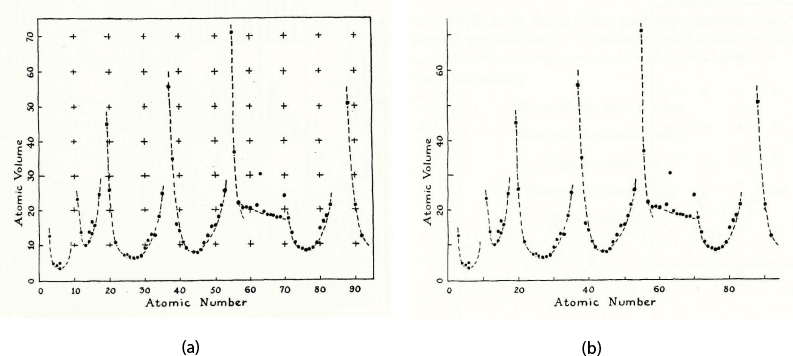
\includegraphics[width=0.8\textwidth]{images/tuftegraphs.png}
\caption{(a) shows the original graph and (b) shows how Tufte recommends changing the graph to remove redundant information}
\label{fig:tuftegraphs}
\end{figure}


Tufte concludes the chapter with 5 maxims summarising this principle.

\begin{verse}Above all else show the data.
	Maximize the data-ink ratio.
	Erase non-data-ink.
	Erase redundant data-ink.
Revise and edit.
\end{verse}

These maxims shall be considered when designing the visualisation of the feedback score.

\subsection{Machine Learning}
The cognitive modelling of students allows can provide access to important information for automatic tutoring systems. A cognitive model is a computer model of the cognitive processes of a student, which allows insight into how the student might approach the problem, or how difficult it might be. Building this model manually requires a lot of human effort\cite{simstudent_better} and so automating this process would be desirable.

SimStudent is a machine learning agent designed to build cognitive models automatically via machine learning. The machine learning method uses for parts of SimStudent is a First Order Inductive Learner, which is given some some observations and some background knowledge from which it draws hypotheses. Using algebra as an example, SimStudent will be given some basic operators as background knowledge (add, subtract etc) and will then be given an algebraic problem to solve. It will then suggest the next step to the student who may reject or accept the suggestion, thus providing negative or positive feedback to SimStudent to modify its production rules.

Providing the students perform consistently, SimStudent can model the performance of the students with an accuracy of 83\%\cite{simstudent}.
